\newif\ifinria
\def\ptitle{Comparaison de métriques de similarité pour la détection de différences dans les logs d'intégration continue} % Title
\def\pauthor{Yamine Belkhedra} % Author
\def\padvisors{Nicolas Hubner} % Advisors
\def\pteam{Bordeaux INP} % Team
\def\pinstitute{Enseirb-Matmeca, LaBRI} % Affiliation
\def\pdate{Jeudi 25 Avril 2024} % Date
\inriafalse % inriatrue/inriafalse to enable/disable Inria logo

\pdfobjcompresslevel=0
\documentclass[final,hyperref={pdfpagelabels=false}]{beamer}
\usepackage[orientation=portrait,size=a0,scale=1.4]{beamerposter}
\usepackage[utf8]{inputenc}
% \usepackage[sfdefault]{roboto}
\usepackage[english]{babel}
\usepackage{amsmath, amsthm, amssymb, array, booktabs, grffile, latexsym, tabularx, xspace}
\newcolumntype{Z}{>{\centering\arraybackslash}X}
\newcommand{\pphantom}{\textcolor{ta3aluminium}}
\newlength{\columnheight}

\def\plogo{logo/logo_em.jpg}
\def\purl{https://github.com/ybelkhedra/annotation-log-line/}

\mode<presentation>{\usetheme{SDSLaBRI}}
\title[\ptitle]{\texorpdfstring{\huge \ptitle}{\ptitle}}
\author[\pauthor]{\pauthor\ -\ \padvisors}
\institute[\pinstitute]{\pteam\ -\ \pinstitute}
\date[\pdate]{\pdate}
\setlogo{\plogo}
\setauthorurl{\purl}


\graphicspath{{./fig/}} % Figures and logos directory
\setlength{\columnheight}{588ex} % Tweak this value if columns are too long/short (should be okay with 588ex)
\newcommand{\pname}{\textsc{Priva-Stream}\xspace} % For demonstration purpose only

\begin{document}
\begin{frame}
  \begin{columns}
    \begin{column}{.49\textwidth}
      \begin{beamercolorbox}[center,wd=\textwidth]{postercolumn}
        \begin{minipage}[T]{.95\textwidth}
          \parbox[t][\columnheight]{\textwidth}{
            
            \begin{block}{Log d'intégration continue}
            
            Définition : L'\textbf{intégration continue} c'est :

            \begin{itemize}
              \item une bonne pratique de développement logiciel (devOps) ;
              \item un processus d'automatisation de l'intégration des changements de code réalisés par plusieurs contributeurs dans un dépôt central ;
              \item un processus d'automatisation de la construction et des tests de l'application.
            \end{itemize}

            Les \textbf{logs d'intégration continue} sont des fichiers textes générés par les outils d'intégration continue qui contiennent des informations sur l'état de l'application, du système, du code, des tests...

            % 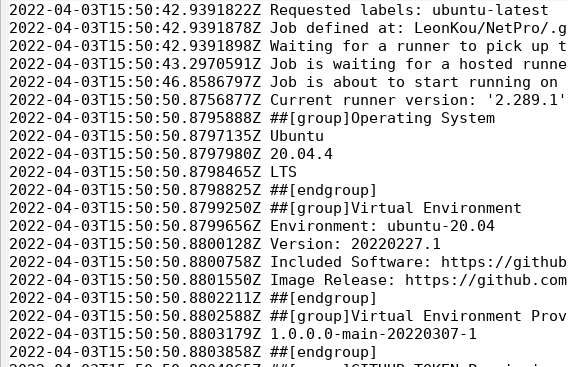
\includegraphics[width=.33\textwidth]{sample/example_log.png}

            \begin{figure}[h!]
              \centering
              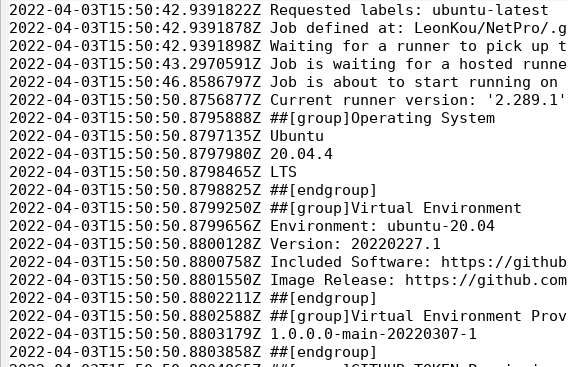
\includegraphics[width=0.5\textwidth]{sample/example_log.png}
              \caption{Exemple de logs d'intégration continue}
              \label{fig:example_log}
          \end{figure}

            \end{block}

            
            \vfill
            
            \begin{block}{Métriques de similarité}
            
            Définition : Une \textbf{métrique de similarité} est une fonction qui mesure la similarité entre deux objets, dans notre cas deux chaînes de caractères.	La valeur peut être comprise entre 0 et 1 :
            \begin{itemize}
              \item 0 signifie que les deux chaînes sont complètement différentes ;
              \item 1 signifie qu'elles sont strictement identiques.
            \end{itemize}

            Application : Les métriques de similarité sont utilisées dans les outils de gestion de version pour détecter les différences entre deux versions d'un fichier texte, et donc de mettre en évidences des lignes ajoutées, supprimées ou modifiées.
            
            \end{block}
            
            \vfill
            
            \begin{block}{Cidiff : métrique développée par le doctorant Nicolas Hubner}
            
            Objectif : Développer une métrique de similarité spécialisée pour les logs d'intégration continue.
            
            \end{block}
            
            \vfill
            
            \begin{block}{Exemples de métriques et de résultats}

              Texte 1 : \texttt{Mon voisin très malin a justement situé une nouvelle planète.}
              \newline
              Texte 2 : \texttt{Mon copain très sympa a justement situé une ancienne exoplanète.}
              \newline
              Texte 3 : \texttt{Bonjour le monde !}
              \newline
              Texte 4 : \texttt{B0nj0ur l3 m0nd3 ?}
            
              \begin{tabular}{|l|c|c|}
                \hline
                \textbf{Métrique} & \textbf{Texte 1 VS Texte 2} & \textbf{Texte 3 VS Texte 4} \\
                \hline
                Python diff distance & 0.79 & 0.67 \\
                Cosine similarity & 0.47 & 0.0 \\
                Levenshtein distance & 0.72 & 0.67 \\
                Smith Waterman distance & 0.66 & 0.67 \\
                Mongel Elkan distance & 0.86 & 0.8 \\
                Jaro Winkler distance & 0.84 & 0.8 \\
                Jaccard distance & 0.78 & 0.6 \\
                Ngram distance & 0.25 & 0.0 \\
                LCS distance & 0.77 & 0.67 \\
                Cidiff distance & 0.8 & 0.0 \\
                \hline
              \end{tabular}
            
            \end{block}
            \vfill
            
          }
        \end{minipage}
      \end{beamercolorbox}
    \end{column}
    \begin{column}{.49\textwidth}
      \begin{beamercolorbox}[center,wd=\textwidth]{postercolumn}
        \begin{minipage}[T]{.95\textwidth}
          \parbox[t][\columnheight]{\textwidth}{
            
            \begin{block}{Fonctionnement de Cidiff}
              
              Permet de comparer deux chaînes de caractères en :
            \begin{itemize}
              \item comparant les chaînes de caractères mot à mot pour calculer un score de similarité ;
              \item attribuant plus ou moins de points selon la ressemblance des mots en utilisant la "longest common subsequence (LCS) distance" ;
            \end{itemize}
            
            \end{block}
            
            \vfill
            
            \begin{block}{Évaluation des performances de Cidiff}
            
            Objectif : Comparer les performances de Cidiff avec d'autres métriques de similarité.

            Protocole :
            \begin{itemize}
              \item Utilisation d'un dataset contenant des fichiers de logs d'intégration continue ;
              \item Création d'un outil d'annotation manuelle de paires de lignes de logs en Python par Yamine Belkhedra ;
              \item Annotations de paires de ligne de logs par Yamine Belkhedra et Nicolas Hubner ;
              \item Calcul des scores de similarité entre les paires de lignes de logs annotées ;
              \item Comparaison des scores de similarité calculés avec les annotations manuelles.
            
            \end{itemize}
            
            \end{block}
            
            \vfill
            
            \begin{block}{Résultats}
              
              \centering
              \begin{tabular}{|l|c|c|c|c|}
                \hline
                \textbf{Metric} & \textbf{Accuracy} & \textbf{Precision} & \textbf{Recall} & \textbf{F1} \\
                \hline
                Cidiff & 0.91 & 0.93 & 0.92 & 0.92 \\
                Python diff & 0.86 & 0.90 & 0.88 & 0.87 \\
                Levenshtein distance & 0.83 & 0.88 & 0.86 & 0.85 \\
                SmithWaterman & 0.86 & 0.90 & 0.88 & 0.87 \\
                MongeElkan & 0.68 & 0.85 & 0.72 & 0.66 \\
                Jarowinkler & 0.69 & 0.85 & 0.73 & 0.68 \\
                Jaccard & 0.82 & 0.88 & 0.84 & 0.83 \\
                Ngram & 0.86 & 0.91 & 0.88 & 0.87 \\
                LCS & 0.81 & 0.87 & 0.83 & 0.83 \\
                Cosine similarity & 0.56 & 0.62 & 0.52 & 0.51 \\
                \hline
              \end{tabular}
              
              \begin{itemize}
              \item Meilleur score F1 :  cidiff 0.92
              \item Meilleur recall :  cidiff 0.92
              \item Meilleur precision :  cidiff 0.93
              \item Meilleur accuracy :  cidiff 0.91
              \end{itemize}
            
            \end{block}
            
            \vfill
            
            \begin{block}{Résultats}
              
              \centering
                  \begin{figure}[h!]
                    \centering
                    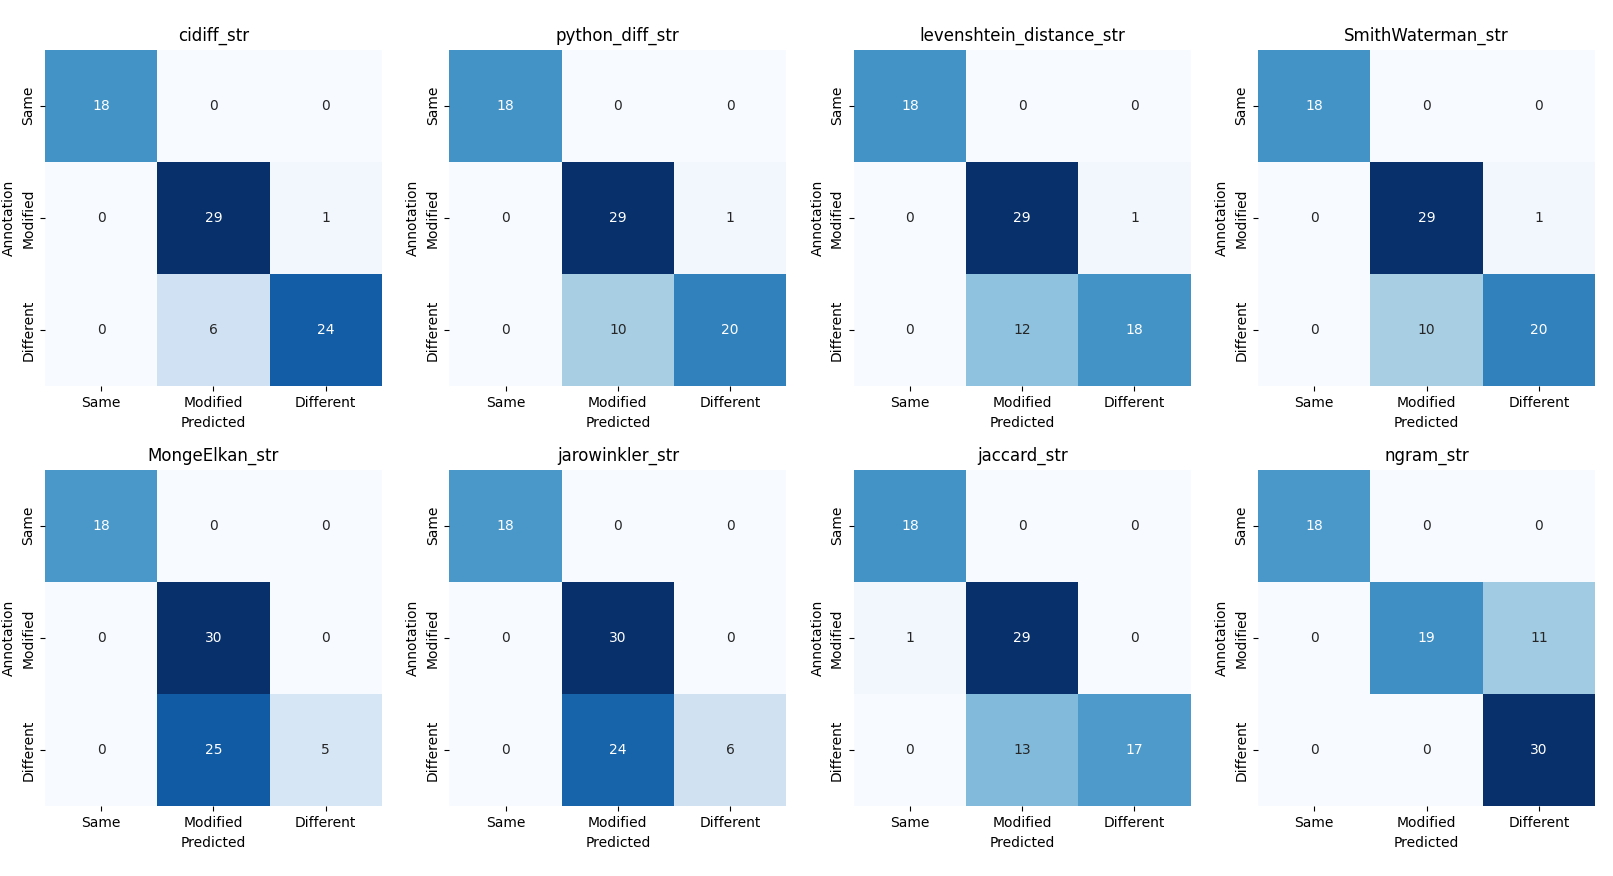
\includegraphics[width=1.0\textwidth]{sample/confusion_matrix.png}
                    \caption{Matrices de confusion des résultats obtenus pour chaque métrique}
                    \label{fig:example_log}
                \end{figure}
            
            \end{block}
            
            \vfill

          }
        \end{minipage}
      \end{beamercolorbox}
    \end{column}
  \end{columns}
  \vskip1ex
\end{frame}
\end{document}
